%****************************************************************
% Chapter X
%****************************************************************
\label{ChapterX}
\chapter{Chapter X}

%****************************************************************
\section{Ray Intersection}

Detect collisions between ray and models is the key to allow user selecting objects in the VR would, which is one of the importent experience for user interaction.

A ray can be describe in a equation with known ray start position \emph{$\overrightarrow{R_0}$} and ray direction \emph{$\overrightarrow{R_d}$}.

\begin{equation}\label{equ:ray-t}
\overrightarrow{R(t)} = \overrightarrow{R_0} + \overrightarrow{R_d} \cdot t
\end{equation}

%****************************************************************
\subsection{Ray-Sphere}

\begin{figure}[H]\label{fig:ray-sphere}
\centering
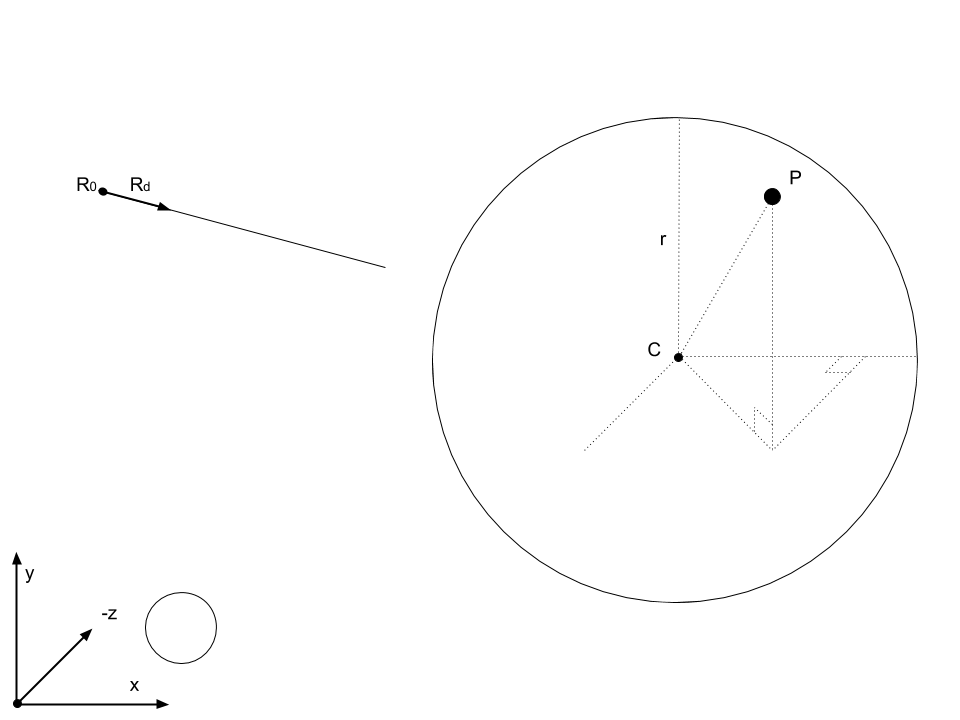
\includegraphics[width=\linewidth]{Figures/ray-sphere-intersection.png}
\decoRule
\caption[ray-sphere-intersection]{Ray-Sphere intersection}
\end{figure}

A point \emph{P} on the surface of sphere should match the equation:

\begin{equation}\label{equ:sphere-surface}
(x_p - x_c)^2 + (y_p - y_c)^2 + (z_p - z_c)^2 = r^2
\end{equation}

If the ray intersects with the sphere at any position\emph{P} must match the equation \ref{equ:ray-t} and \ref{equ:sphere-surface}. Therefor the solution of \emph{t} in the cointegrate equation implies whether or not the ray will intersect with the sphere:

\[
\begin{aligned}
(x_{R_0} + x_{R_d} \cdot t - x_c)^2 + (y_{R_0} + y_{R_d} \cdot t - y_c)^2 + (z_{R_0} + z_{R_d} \cdot t - z_c)^2 &= r^2 \\
&\vdots \\
x_{R_d}^2 \cdot t^2 + (2 \cdot x_{R_d} \cdot (x_{R_0} - x_c)) \cdot t + (x_{R_0}^2 - 2 \cdot x_{R_0}\cdot x_c + x_c^2) & \\
+\,y_{R_d}^2 \cdot t^2 + (2 \cdot y_{R_d} \cdot (y_{R_0} - y_c)) \cdot t + (y_{R_0}^2 - 2 \cdot y_{R_0}\cdot y_c + y_c^2) & \\
+\,z_{R_d}^2 \cdot t^2 + (2 \cdot z_{R_d} \cdot (z_{R_0} - z_c)) \cdot t + (z_{R_0}^2 - 2 \cdot z_{R_0}\cdot z_c + z_c^2) &= r^2
\end{aligned}
\]

It can be seen as a quadratic formula:

\begin{equation}\label{equ:sphere-surface-quadratic-formula}
a \cdot t^2 + b \cdot t + c = 0
\end{equation}

At this point, we are able to solved the \emph{t}:

\[
t =
\begin{cases}
\frac{-b \pm \sqrt{b^2 - 4ac}}{2a} & \text{if } b^2 - 4ac > 0 \\
\frac{-b}{2a} & \text{if } b^2 - 4ac = 0 \\
\varnothing & \text{if } b^2 - 4ac < 0
\end{cases}
\]

Then, I take a further step to get rid of formula complexity.

$\because$ Equation \ref{equ:sphere-surface},\,\ref{equ:sphere-surface-quadratic-formula}
\[
\left\{
\begin{array}{lr}
a = x_{R_d}^2 + y_{R_d}^2 + z_{R_d}^2 \\
b = 2 \cdot (x_{R_d} \cdot (x_{R_0} - x_c) + y_{R_d} \cdot (y_{R_0} - y_c) + z_{R_d} \cdot (z_{R_0} - z_c)) \\
c = (x_{R_0} - x_c)^2 + (y_{R_0} - y_c)^2 + (z_{R_0} - z_c)^2 - r^2
\end{array}
\right.
\]

$\And$
\[
\begin{array}{lr}
\begin{aligned}
\norm{\overrightarrow{R_d}} &= \sqrt{x_{R_d}^2 + y_{R_d}^2 + z_{R_d}^2} = 1 \\
\overrightarrow{V_{c\_R_0}} &= \overrightarrow{R_0} - \overrightarrow{C} = \overrightarrow{(x_{R_0} - x_c,\,y_{R_0} - y_c,\,z_{R_0} - z_c)}
\end{aligned}
\end{array}
\]

$\therefore$
\[
\left\{
\begin{array}{lr}
a =1 \\
b = 2 \cdot \overrightarrow{R_d} \cdot \overrightarrow{V_{c\_R_0}} \\
c = \overrightarrow{V_{c\_R_0}} \cdot \overrightarrow{V_{c\_R_0}} \cdot r^2
\end{array}
\right.
\]

$\because$ The formula for \emph{t} can also be optimized
\[
\left\{
\begin{array}{lr}
\frac{-b \pm \sqrt{b^2 - 4ac}}{2a} = -\alpha \pm \sqrt{\beta} \\
\alpha = 0.5b \\
\beta = \alpha^2 - c
\end{array}
\right.
\]

$\therefore$ This is the final solution for \emph{t}
\[
t =
\begin{cases}
 -\alpha \pm \sqrt{\beta} & \text{if } \beta > 0 \\
-\alpha & \text{if } \beta = 0 \\
\varnothing & \text{if } \beta < 0
\end{cases}
\]

And the collision position for each \emph{t} is:

\[
\overrightarrow{P} = \overrightarrow{R_0} + \overrightarrow{R_d} \cdot t
\]

%****************************************************************
\subsection{Ray-Plane}

\begin{figure}[H]\label{fig:ray-plane}
\centering
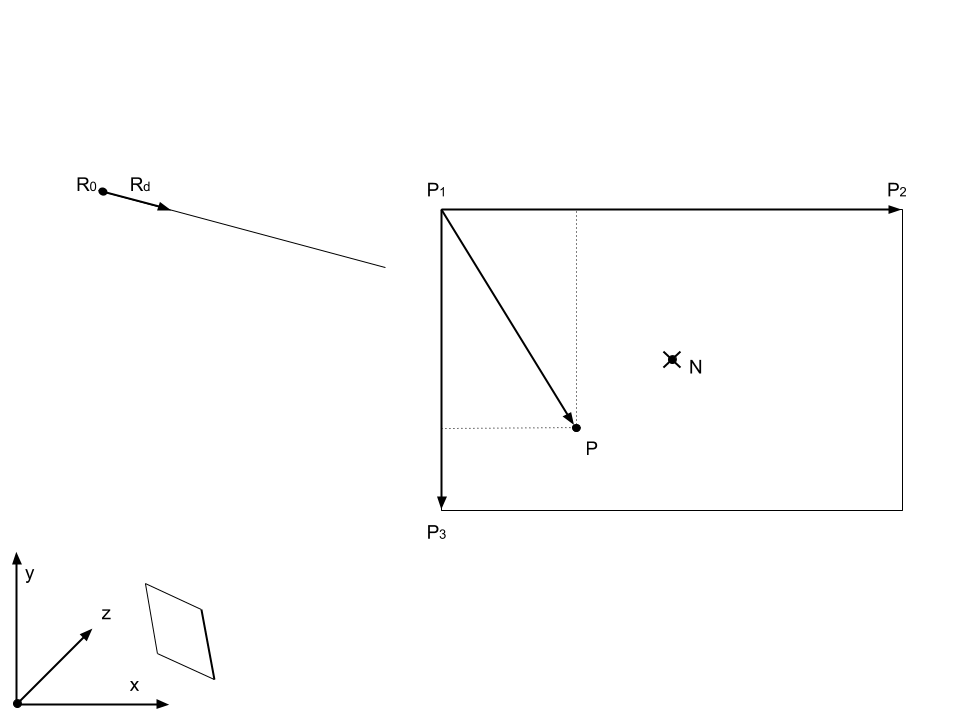
\includegraphics[width=\linewidth]{Figures/ray-plane-intersection.png}
\decoRule
\caption[ray-plane-intersection]{Ray-Plane intersection}
\end{figure}

If a point \emph{P} on the plane and also belongs to the ray, we have quadric equation:

\begin{equation}\label{equ:ray-plane-intersection}
\left\{
\begin{array}{lr}
(\overrightarrow{P} - \overrightarrow{S_1}) \cdot \overrightarrow{N} = 0 \\
\overrightarrow{P} = \overrightarrow{R_0} + \overrightarrow{R_d} \cdot t
\end{array}
\right.
\end{equation}

Solution for the \emph{t} is:

\[
t =
\begin{cases}
\frac{-\overrightarrow{N} \cdot (\overrightarrow{R_0} - \overrightarrow{S_1})}{\overrightarrow{N} \cdot \overrightarrow{R_d}} & \text{if } \overrightarrow{N} \cdot \overrightarrow{R_d} \nsim 0 \\
\varnothing & \text{if } \overrightarrow{N} \cdot \overrightarrow{R_d} \sim 0
\end{cases}
\]

At last, we have to verify if the collision is inside of the quadrangle by putting \emph{t} back to \ref{equ:ray-plane-intersection}, and the \emph{t} is valid only if:

\[
\begin{array}{lr}
\mu = \sqrt{(\overrightarrow{P} - \overrightarrow{S_1}) \cdot (\overrightarrow{S_2} - \overrightarrow{S_1}))} \in [\,0,\,\norm{\overrightarrow{S_2} - \overrightarrow{S_1}}\,] \\
\nu = \sqrt{(\overrightarrow{P} - \overrightarrow{S_1}) \cdot (\overrightarrow{S_3} - \overrightarrow{S_1}))} \in [\,0,\,\norm{\overrightarrow{S_3} - \overrightarrow{S_1}}\,] 
\end{array}
\]

%****************************************************************
\subsection{Ray-Box}

There is a octree implementation in the VR 3D world that separate the 3D world to 3D boxes to avoid unnecessary ray-object collision detection. In this section, I am going to first explain Ray-Box-2D collision detection, then derive out Ray-Box-3D intersection.

%****************************************************************
\subsubsection{Ray-Box-2D}

\begin{figure}[H]\label{fig:ray-box-2d}
\centering
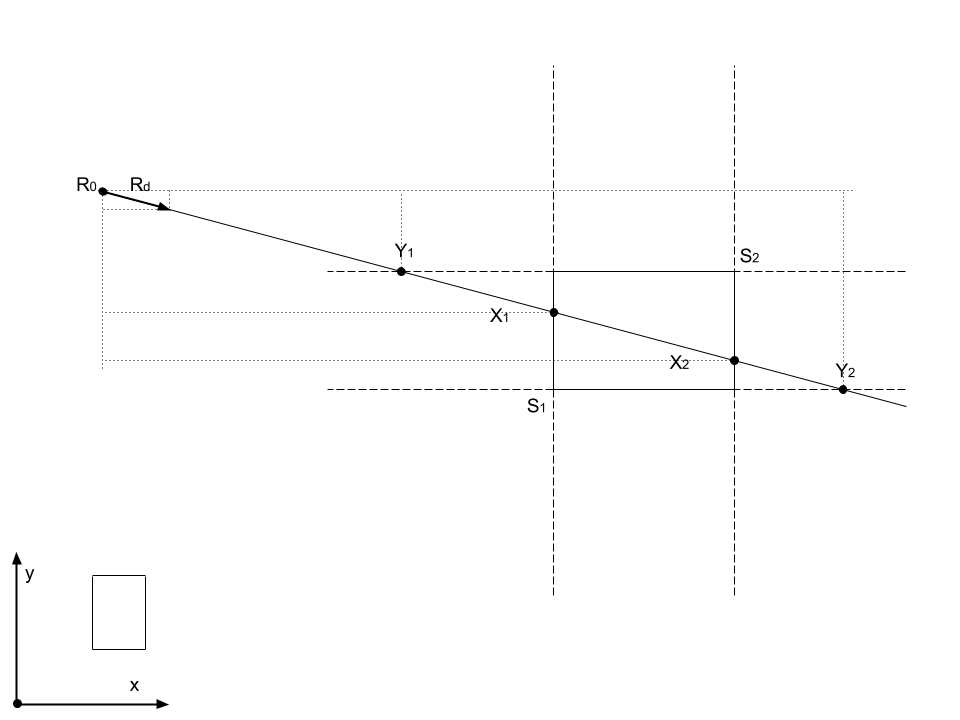
\includegraphics[width=\linewidth]{Figures/ray-box-2d-intersection.png}
\decoRule
\caption[ray-box-2d-intersection]{Ray-Box-2D intersection}
\end{figure}

$\because$ Known $R_0$,\,$R_d$,\,$S_1$,\,$S_2$
\begin{multicols}{2}
\noindent
\[
X_1 =
\begin{cases}
x_{S_1} - x_{R_0} & \text{if } x_{R_d} > 0 \\
x_{S_2} - x_{R_0} & \text{if } x_{R_d} < 0
\end{cases}
\]
\[
X_2 =
\begin{cases}
x_{S_2} - x_{R_0} & \text{if } x_{R_d} > 0 \\
x_{S_1} - x_{R_0} & \text{if } x_{R_d} < 0
\end{cases}
\]
\[
\begin{array}{lr}
t_{X_1} = \frac{X_1}{x_{R_d}} \\
t_{X_2} = \frac{X_2}{x_{R_d}}
\end{array}
\]
\columnbreak
\[
Y_1 =
\begin{cases}
y_{S_1} - y_{R_0} & \text{if } y_{R_d} > 0 \\
y_{S_2} - y_{R_0} & \text{if } y_{R_d} < 0
\end{cases}
\]
\[
Y_2 =
\begin{cases}
y_{S_2} - y_{R_0} & \text{if } y_{R_d} > 0 \\
y_{S_1} - y_{R_0} & \text{if } y_{R_d} < 0
\end{cases}
\]
\[
\begin{array}{lr}
t_{Y_1} = \frac{Y_1}{y_{R_d}} \\
t_{Y_2} = \frac{Y_2}{y_{R_d}}
\end{array}
\]
\end{multicols}

$\And$ When collision happens,  we have formula
\[
\left\{
\begin{array}{lr}
\begin{aligned}
t_{X_1} &< t_{X_2} \\
t_{Y_1} &< t_{Y_2}
\end{aligned}
\end{array}
\right.
\]

$\therefore$ Which is
\begin{equation}\label{equ:ray-box-2d-intersection}
max(t_{X_1},\,t_{Y_1}) < min(t_{X_2},\,t_{Y_2})
\end{equation}

%****************************************************************
\subsubsection{Ray-Box-3D}

\begin{figure}[H]\label{fig:ray-box-3d}
\centering
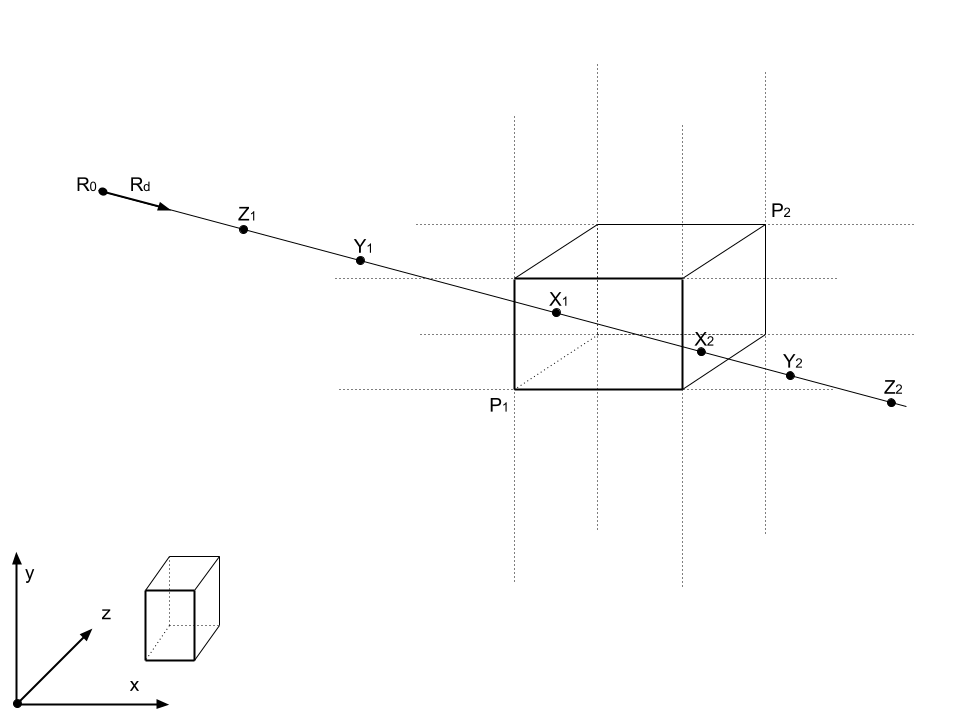
\includegraphics[width=\linewidth]{Figures/ray-box-3d-intersection.png}
\decoRule
\caption[ray-box-3d-intersection]{Ray-Box-3D intersection}
\end{figure}

asdasd



%****************************************************************
\section{Section 2}
asdasd

\subsection{Subsection 1}
asdasdasd

\subsection{Subsection 2}
asdasdasdasd

%****************************************************************
\section{Section 3}

\subsection{Subsection 1}
asdasdasd

\subsection{Subsection 2}
asdasdasdasd

\subsection{Subsection 3}
asdasdasd

%****************************************************************
\section{Section 4}

